\section{Basic Data Science Techniques}
These next few sections serve to provide background into key tools we used in our methodology. These data science techniques are commonly employed for the type of classification problem we have. To learn more about these tools, we delve first into machine learning, then decision trees and finally random forests. 

\subsection{A Brief Overview of Machine Learning}
Machine learning is a field of applied mathematical statistics and analytics where computers are used to model the behavior of datasets in ways human minds cannot perceive. Machine learning has a wide range of applications from computer vision to weather forecasting. These methods rely on the use of known sample data, which is split into two non-overlapping data subsets: training and testing. The training set is fed to the learner, enabling it to identify trends and patterns in the data. The testing set is used to validate how predictive the learned trends were. These two sets should be completely distinct (share no data points between them) as the efficacy of prediction on the training set does not reflect the efficacy of prediction on future data. For this application, we are concerned with predicting the success of online fantasy sport contests hosted by DraftKings. 

%This falls under the domain of supervised learning classification, because for our set, we can determine if a contest fills or not.

Supervised learning is a form of machine learning where both the inputs and outputs are known in the sample data (i.e. all data is labeled). Entry $i$ of this set would come in the form of

\begin{equation}
    (X_{i}, y_{i}) = (x_{1i}, x_{2i}, \cdots, x_{ji}, y_{i}), \quad X\in{\rm I\!R}^{n\times j}, \quad y\in{\rm I\!R}^{n}
\end{equation}

%where is this notation from? 

where $y_{i}$ is the response value and $x_{ji}$ is the $j^{th}$ feature.

Supervised learning aims to generate a function which can map from a set of features $X$ to a set of estimated responses $\hat{y}$ where $\hat{y}$ is consistently as close to the true responses $y$ as possible. When the label is a finite set of discrete categories, this is known as classification. In our dataset, each contest can be labeled "Success" if it completely fills or "Failure" if it does not which is a form of binary classification (classification into two possible categories).

While one function mapping the features to a response can be effective, a system of functions can often be even better. Ensemble learning is a machine learning technique which uses multiple weaker learners in parallel to collectively output a new, stronger prediction than any single learner could. Errors are reduced in ensemble learning because of the nature of the collection. If a single model makes an error based on the limited data it has, that error can be easily corrected by numerous other models which have other data. In this way, by measuring averages rather than individual results, an ensemble can be more effective for predictive modeling than any one technique.

\subsection{Decision Trees}
Random Forests are one example of ensemble learning, utilizing many decision trees as their predictors, however, one must first understand the Decision Tree algorithm. Recall that for this application of supervised learning, there are a number of features and one binary response variable for each entry. A sample data set can be seen in Table \ref{tab:headfill} for a binary classification problem like this. To simplify the example, consider a data set with only two features and a binary categorical response variable, as appears in Figure \ref{fig:dectrees}.

In Figure \ref{fig:dectrees}, we see a set of 20 randomly generated points in 2-dimensional space, each classified as either a success or a failure. The goal of a decision tree is to draw vertical or horizontal separators that minimize the number of incorrect classifications. Again referring to our example, we first draw a horizontal line around $x=.25$ and classify everything less than that value as a failure and everything right of that value a success. This results in a mis-classification of 7 points, the fewest of any line we could have drawn. The next branch we make in our decision tree is a horizontal line at $y=.3$, classifying everything below the line a success and everything above it as a failure. This results in four mis-classifications, again the fewest of any possible line. We can continue creating these cuts until a region only has one point. This example can also be extended to a case with more than two features, but a cut can only ever be along one axis. \newline 

\begin{table}
\centering
\begin{tabular}{| c | c | c | c | c |}
\hline
\textbf{Contest ID} & \textbf{EntryFeeAmount} & \textbf{TopPrize} & \dots & \textbf{Response} \\ 
\hline
1932122 & 5.0 & 1000.0 & \dots & Success \\  
\hline
2494993 & 2.0 & 650.0 & \dots & Failure \\
\hline
\vdots & \vdots & \vdots & \ddots & \vdots \\
\hline
\end{tabular}
\caption[Example Binary Response Dataset]{A sample binary response dataset similar to our actual dataset. Note the actual dataset includes 21 columns of the features listed in Table \ref{tab:headercols} and has over 600,000 entries.}
\label{tab:headfill}
\end{table}

\begin{figure}
\centering
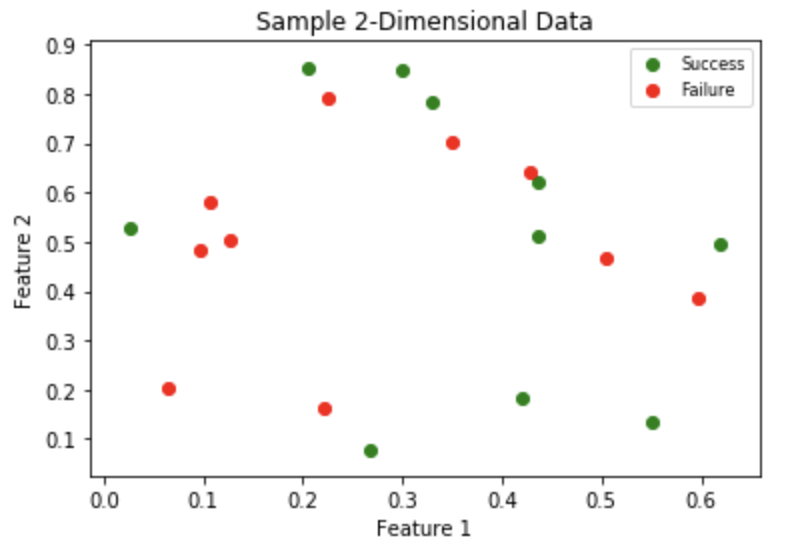
\includegraphics[width=6cm]{body/background/ogtree.png}
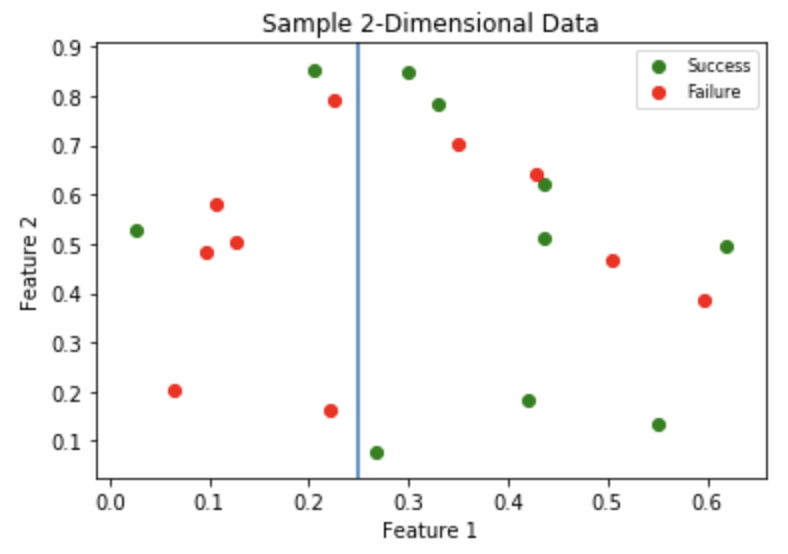
\includegraphics[width=6cm]{body/background/tree2.png}
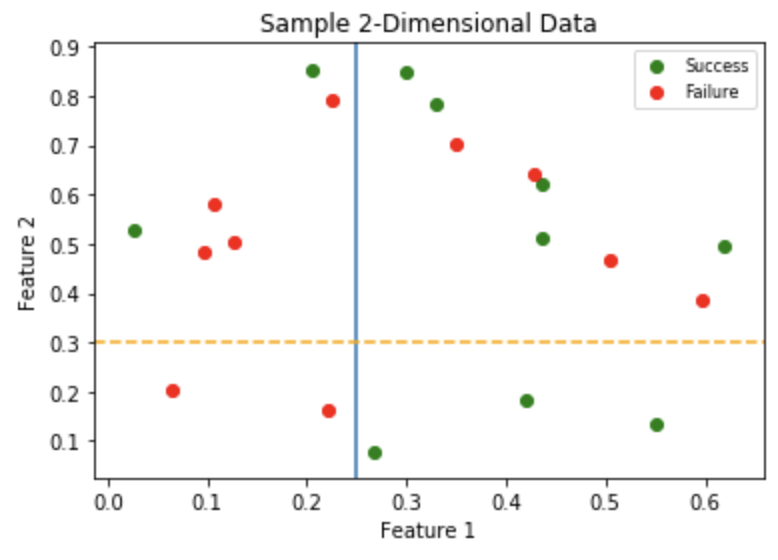
\includegraphics[width=6cm]{body/background/tree3.png}
\caption[Sample Decision Tree Classifier]{Sample set of 2-dimensional binary response data with two possible initial decision tree splits marked. In the top left image, we have only the data points. In the top right, the algorithm makes the cut that mis-classifies the fewest number of points, at $x=2.5$, classifying points with $x$ values less than that as failures and greater as successes. The bottom picture is the second cut, again minimizing the mislabeled points. This process could continue until we only have regions with one point.}
\label{fig:dectrees}
\end{figure}

Tree learning centers on using known features ($X$) of the dataset to section the predictive space into distinct regions. Looking at the example dataset in Figure \ref{fig:dectrees}, we can see 

$$X = (\bm{x_{1}}, \bm{x_{2}}), \quad \bm{y}\in[Success, Failure]$$

A line could be superimposed on Figure \ref{fig:dectrees} where $x_{1} = 0.25$. Then based on the sample data, we could predict that any point where $x_{1} < 0.25$ should be a Failure. By repeatedly adding linear separators, it becomes possible to create multiple areas of classification. The question then becomes determining how to best split the space.

In our example, we start by partitioning the left most points because that cut limits the number of mis-classifications. A common way of choosing splits for classification is the use of Gini Impurity (GI). Gini Impurity is a metric for the uniformity of response types in a region calculated by

%it is alone and therefore an easy opportunity to instantly create a region of a single response type on the left. However, consider the case where a new failure occurs when $x1 = 2$ and $x2 = 6$. Now, there are no easy splits that can be made to create unanimous areas. 

\begin{equation}
    GI = \sum_{c} p(y = c | x_{i})(1 - p(y = c | x_{i}))
\end{equation}

where $p(y = c | x_{i})$ is the conditional probability of a point in a region being of response type $c$ given some feature $x_{i}$. Similarly, $1 - p(y = c | x_{i})$ is the conditional probability of a point in a region not being of response type $c$ given feature $x_{i}$. For a given region $R$, $p(y = c | x_{i})$ can be calculated as the percent of elements within $R$ of class $c$, meaning $1 - p(y = c | x_{i})$ is the percent of elements in $R$ not of class $c$.

As the regions become more uniform, the impurity value decreases, eventually approaching 0 when all points in the region are of the same type. It it then possible to select the next split that best separates the data in one of the new regions by minimizing the sum of the Gini Impurities on either side of the new split.

In our example, we only consider the classes $c_{1} = Success$ and $c_{2} = Failure$. Since this is a binary classification, $(1 - p(y = Failure | x_{i})) = p(y = Success | x_{i}))$ and vice versa. Substituting this into Equation 2.2 and simplifying, we find

\begin{equation}
    GI = 2p(y = Success | x_{i})p(y = Failure | x_{i}))
\end{equation}

From this, we can see that splitting at $x_{1} = 0.25$ produces the lowest impurity sum and is thus the best option. A tree can then be formed from all splits in the order they were made to evaluate new data points to decide whether they will be a "Success" or "Failure".

%The final set of splits could appear as in figure 2.4, producing a final learned tree like the one in figure 2.5.

%\begin{figure}
%\centering
%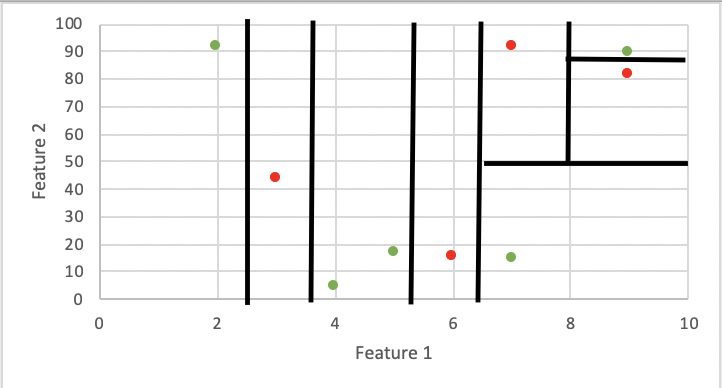
\includegraphics[width=8cm]{body/background/cuttree.png}
%\caption{Forest Segmentation}
%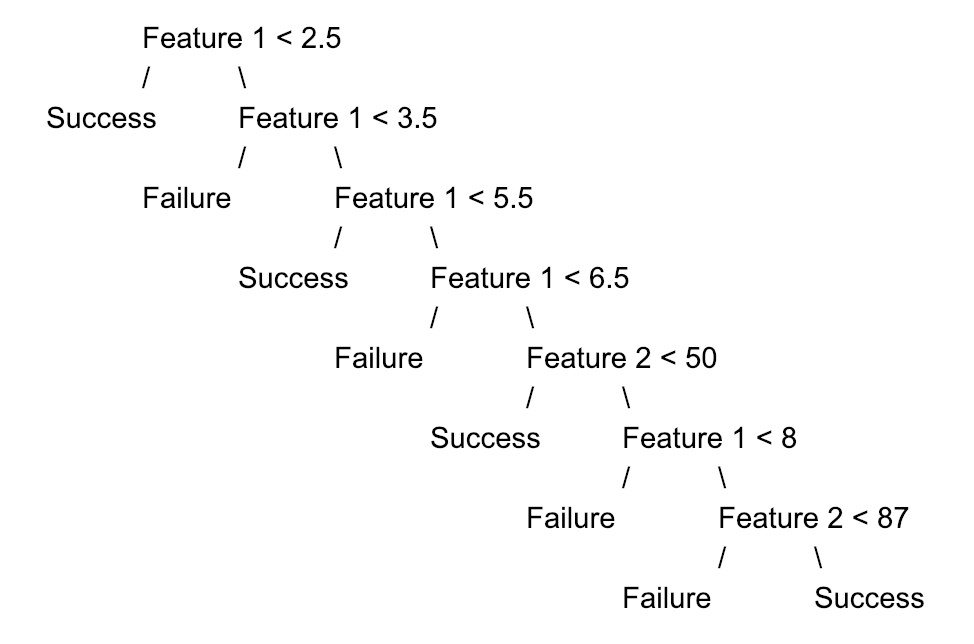
\includegraphics[width=8cm]{body/background/decisiontree.png}
%\caption{Forest Tree Diagram}
%\end{figure}

%In this model, it should be noted that only one feature may be considered for each branching split. At each iteration, we may only break along the axis of Feature 1 or Feature 2, not along some diagonal dependent on both. This example is easily extended to the multidimensional case with more than two features, as the algorithm will first find the break along any feature $x_{i}$ axis that reduces the gini impurity. 
We can also use decision trees for regression problems, where we would predict a numerical response at each cut, but for the purposes of this project, we need only consider the classification application.

%Dont like how this paragraph is organized. I think it should be: Decision trees are bad because overfitting, explain why. Random forests fix this becuase they break up the features into smaller chucks.
A decision tree that uses all the features and can make as many branches as possible is likely to overfit, or build its predictions too closely off of the training data. This can be detrimental for predicting as the overfitted tree will likely do well on the trained set and poorly on new data points in the testing set. Several techniques have been developed to prevent overfitting of decision trees including limiting the number of features provided to the algorithm and the number of branches (linear separators) it can produce. While a stunted tree such as this can help reduce overfitting, they are also prone to inaccuracy. To improve the predictive capabilities of this algorithm, it is common to use multiple stunted trees in parallel to form an aggregate prediction. The issue then becomes deciding how to effectively limit the features and branching of each tree.

\subsection{The Random Forest Algorithm}
The Random Forest algorithm is an ensemble learning method for supervised learning problems in data science. The algorithm utilizes multiple randomly selected features in decision trees in order to predict outputs making it both easily implementable and interpretable. While random forests can be used for both regression and classification, for the purposes of this paper, we will only discuss classification.

A Random Forest is a supervised technique using a collection of many decision trees where each tree has approximately $k$ features, randomly selected from all $n$ features, $k \leq n$. An important methodology to implement random forests is called bagging, or bootstrap aggregation. Bootstrapping is the process by which a random sample is taken from the dataset for each model used in the ensemble. Each bootstrapped sample has the same number of elements $n$ selected with replacement. This means each element in a bootstrap sample is selected randomly from the original data set without deleting it from the original set. This also ensures that each bootstrap preserves the approximate distribution of the original set. Thus, the general form of the data is maintained across all bootstraps.

As an example, consider a random forest of 1000 decision trees where each tree receives a different bootstrapped sample set. A common implementation would split the trees into 10 equal batches of 100. Each batch would then have its branching limited by a different integer, creating an ensemble of trees with varying levels of complexity. Each tree ($t$) then gets a ``vote'' (weighted equally in most cases) as to the categorization of each point. The category receiving the majority vote from the set of all trees (T) is then predicted as the proper class. 

$$\rm{v} = \frac{\sum_{i = 1}^n {\rm I\!I}_{i}(t_{i} = Success)}{|T|}$$ 
\[ {\rm I\!I}_{i} =  \begin{cases} 
      1, & t_{i} = Success \\
      0, & \rm{otherwise}
   \end{cases}
\]

\[ \rm{Prediction} =  \begin{cases} 
      Success, & \rm{v}\geq0.5 \\
      Failure, & \rm{otherwise}
   \end{cases}
\]

So, if 500 or more of the 1000 decision trees in our forest predict a point to be a success, it would be classified as a success.

The idea of bootstrapping may seem strange as it means each tree can receive vastly different datasets, each of which may contain duplicate values. In fact, this sampling scheme ultimately improves the modeling performance by ensuring each tree is trained on different data. If each tree were trained on the same original dataset, the splits (and therefore predictive trends) would be similar or identical. This defeats the purpose of the random forest, as having many trees ``voting'' would be pointless if they always tend to vote the same. By bootstrapping, we ensure each tree receives a unique set of training data that is still representative of the original set allowing for decreased variance without increasing the bias of the model.

% As far as training and testing procedure, we would typically divide the original data into training data and testing data with a 75/25 or 80/20 split. We would use the training data to build the random forest of decision trees with the lowest amount of error. Then, using the splits that these trees generate, we compare the testing data sorted via those branches to the actual success and failures, which we know because this is a supervised learning technique. Finally, we can generate a ROC curve or a confusion matrix to measure the accuracy of this model.

\subsection{Advantages and Disadvantages}
One distinct advantage of random forests is their flexibility. Forests are a non-parametric modeling technique, meaning they make no assumptions of the form of the data and therefore can work well for more complex sets of higher dimensional data. However, this comes at a cost. Due to their flexibility, random forests provide no insights into the nature of the data as trends cannot be discerned between features and the output response types, as opposed to a simple decision tree (Donges, 2018). Additionally, depending on the complexity and number of trees, random forests can be computationally costly and are still at risk of overfitting. 
% (add source)